\documentclass[]{article}
\usepackage[top=1in, bottom=1.25in, left=1.25in, right=1.25in]{geometry}
\usepackage{hyperref}
\usepackage{amsfonts}
\usepackage{amsmath}
\usepackage{graphicx}
\usepackage{float}
\usepackage{bbm}

\usepackage{listings}
\usepackage{color}

\definecolor{dkgreen}{rgb}{0,0.6,0}
\definecolor{gray}{rgb}{0.5,0.5,0.5}
\definecolor{mauve}{rgb}{0.58,0,0.82}

\lstset{frame=tb,
	language=Python,
	aboveskip=3mm,
	belowskip=3mm,
	showstringspaces=false,
	columns=flexible,
	basicstyle={\small\ttfamily},
	numbers=none,
	numberstyle=\tiny\color{gray},
	keywordstyle=\color{blue},
	commentstyle=\color{dkgreen},
	stringstyle=\color{mauve},
	breaklines=true,
	breakatwhitespace=true,
	tabsize=3
}

\title{\textbf{Classifiers}}
\author{Yacine Debbabi}

\begin{document}

\maketitle

\tableofcontents

\section{Bayes classifier}

Consider $n$ observations with features $X \in R^{n\times p}$ and their associated unique labels $(g_i)_{i=1}^n\in{1,...,K}^n$. We aim to build a classifier function minimizing the expected prediction error
\begin{equation}
\hat{G}=\mathrm{argmax}_G \mathbb{E}\left[L(g,G(X)\right]
\end{equation}
where $L$ is a $K\times K$ loss matrix. That objective function can be expressed pointwise with a 0-1 loss function as
\begin{eqnarray}
\mathbb{E}\left[L(g,G(X)|X=x\right] &=& \sum_{k=1}^K L(g_k,G(x))\mathbb{P}(g_k|x) \\
&=&1-\mathbb{P}(G(x)|x)
\end{eqnarray}
The solution, called the Bayes classifier, is given by
\begin{equation}
\hat{G}(x)=\mathrm{argmax}_g \mathbb{P}(g|x),
\end{equation}
and its error rate is called the Bayes rate. Several classifiers are constructed by approximating the conditional class probability.

\section{Baseline estimators}

\noindent Simple error rate baselines can be obtained by testing dummy prediction strategies. These include (a) "most\_frequent", i.e. always predict the most frequent class, (b) "uniform", i.e. generates predictions uniformly at random. Such strategies are implemented in "DummyClassifier".

\begin{lstlisting}
from sklearn.dummy import DummyClassifier

dc = DummyClassifier(strategy="most_frequent").fit(X, y)
dc.score(X, y) # accuracy measure, i.e. % of observations classified correctly
\end{lstlisting}

\noindent With multiple classes, one can train binary classifiers to distinguish between a given class and the rest of the classes (\textbf{one-versus-all/rest}), or between two classes (\textbf{one-vs-one}). We usually focus on one-vs-all classifiers and identify the highest score to make a class prediction. \\

\noindent Stratified KFold helps with generating class-balanced sets \href{https://scikit-learn.org/stable/modules/generated/sklearn.model_selection.StratifiedKFold.html#sklearn.model_selection.StratifiedKFold}{here}

\section{Logistic regression}

The model specifies the log-odds of the $K$ classes via linear functions of $x$
\begin{eqnarray}
\log \frac{\mathbb{P}(G=k|X=x)}{\mathbb{P}(G=K|X=x)}=\beta_k^0+\beta_k^Tx,
\end{eqnarray}
ensuring that all class probabilities sum to 1. The model is usually fit by maximum likelihood, i.e. by maximizing the log-likelihood
\begin{eqnarray}
l(\beta)=\sum_{i=1}^n \log p_{g_i}(x_i; \beta).
\end{eqnarray}
When $K=2$, we code the two classes via 0/1 response, so the log-likelihood can be rewritten as
\begin{eqnarray}
l(\beta)&=&\sum_{i=1}^n y_i\log p_{g_i}(x_i; \beta)+(1-y_i)\log\left( 1-p_{g_i}(x_i; \beta)\right)\\
&=&\sum_{i=1}^n y_i\beta^T x_i-\log\left(1+e^{\beta^T x_i}\right)
\end{eqnarray}
where the intercept is accounted for by adding a constant feature equal to 1. Note the log-likelihood is concave; this can be seen by differentiating against $x_i$ twice. \\

\noindent The relevance of features can be examined via the logistic regression Z-scores; see below.

\begin{lstlisting}
import statsmodels.api as sm

X = df[["Pclass", "Sex_"]].values
y = df.Survived

X_ = sm.add_constant(X)
lr = sm.Logit(y, X_)
lr_res = lr.fit()

print(lr_res.summary())

                           Logit Regression Results                           
==============================================================================
Dep. Variable:               Survived   No. Observations:                  891
Model:                          Logit   Df Residuals:                      888
Method:                           MLE   Df Model:                            2
Date:                Sun, 06 Dec 2020   Pseudo R-squ.:                  0.3029
Time:                        09:16:16   Log-Likelihood:                -413.60
converged:                       True   LL-Null:                       -593.33
Covariance Type:            nonrobust   LLR p-value:                 8.798e-79
==============================================================================
coef    std err          z      P>|z|      [0.025      0.975]
------------------------------------------------------------------------------
const          3.2946      0.297     11.077      0.000       2.712       3.878
x1            -0.9606      0.106     -9.057      0.000      -1.168      -0.753
x2            -2.6434      0.184    -14.380      0.000      -3.004      -2.283
==============================================================================
\end{lstlisting}

\noindent Note the coefficient standard errors used to compute the Z-scores are derived using the asymptotic distribution of MLE coefficient estimates, i.e. 
\begin{equation}
\sqrt{n}(\hat{\beta}_{\mathrm{MLE}}-\beta)\rightarrow N(0,I^{-1}),
\end{equation}
where $I$ is the Fisher information matrix defined by
\begin{equation}
I_{j,k}:=\mathbb{E}\left[-\frac{\partial^2 \ln f(X;\beta)}{\partial\beta_j \partial\beta_k} \right].
\end{equation}


\section{Linear discriminant analysis}

This classifier is built as a Bayes classifier by assuming $X|G=k\sim N(\mu_k, \Sigma)$. Note the covariance does not vary with the class. The conditional class probabilities are estimated with the Bayes rule as
\begin{equation}
\mathbb{P}(G=k|x)=\frac{f_k(x)\Pi_k}{\sum_{g=1}^K f_g(x)\Pi_g},
\end{equation}
and we assign the class with highest probability of occurence conditional on $X=x$. Taking the log ratio of two class probabilities shows the decision boundary is linear, i.e.
\begin{eqnarray}
\log \frac{\mathbb{P}(G=k|X=x)}{\mathbb{P}(G=l|X=x)}&=&\log\frac{f_k(x)}{f_l(x)}+\log\frac{\pi_k}{\pi_l}\\
&=&\log\frac{\pi_k}{\pi_l}-\frac{1}{2}(\mu_k+\mu_l)^T\Sigma^{-1}(\mu_k-\mu_l)+x^T\Sigma^{-1}(\mu_k-\mu_l).
\end{eqnarray}
The means and covariance matrix are directly estimated from the data. This makes the techniques sensitive to outliers. The classification is equivalent to computing distances to cluster means in a transformed space. Distances orthogonal to the $K-1$-dimension affine subspace where the $K$ cluster centers lie are irrelevant. This suggests dimensionality can be reduced by projecting the data onto that affine space. That projection can be arrived to following the Fisher decomposition described below. COMPLETE INFO TO LINK THE TWO TECHNIQUES.\\

\noindent The Fischer decomposition consists of finding a sequence of orthonormal directions where the between-class variance is maximized relative to the within-class variance, i.e.
\begin{equation}
\mathrm{argmax}_a \frac{a^T B a}{a^T W a},
\end{equation}
where the between-class and within-class variance are given by
\begin{eqnarray}
B&=&\sum_{g=1}^K N_g (\bar{x}_g-\bar{x})^T (\bar{x}_g-\bar{x}), \\
W&=&\sum_{g=1}^K \sum_{g_i=g} (x_i-\bar{x}_g)^T (x_i-\bar{x}_g).
\end{eqnarray}

\begin{lstlisting}
import seaborn as sns
from sklearn.discriminant_analysis import LinearDiscriminantAnalysis

clf = LinearDiscriminantAnalysis().fit(X, y)
df[["C1","C2"]] = clf.transform(X) # coordinates in the Fisher directions

sns.scatterplot(x='C1', y='C2', data=df, hue='Species')
plt.show()
\end{lstlisting}

\noindent More information on LDA can be found \href{https://www.doc.ic.ac.uk/~dfg/ProbabilisticInference/old_IDAPILecture15.pdf}{here}.

\section{Performance measures}

Let us denote $TP$, $FP$, $TN$ and $FN$ the number of true positives, false positives, true negatives and false negatives. To build some intuition, we consider the detection of a sickness via a test (+$|$-). We define the precision, i.e. P(sick$|$+), as
\begin{equation}
P=\frac{TP}{TP+FP},
\end{equation}
the recall / true positive rate, i.e. P(+$|$sick), as
\begin{equation}
R=\frac{TP}{TP+FN},
\end{equation}
and the false positive rate, i.e. P(+$|$healthy) as
\begin{equation}
\mathrm{FPR}=\frac{FN}{FP+TN}.
\end{equation}

\begin{figure}[H]
	\centering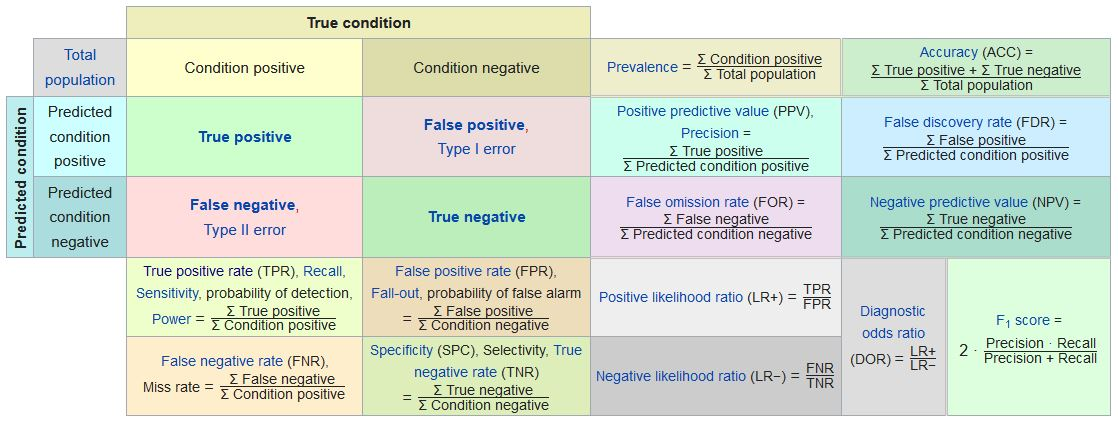
\includegraphics[scale=0.5]{classifier_metrics}
	\caption{Performance metrics summary; from \href{https://en.wikipedia.org/wiki/Receiver_operating_characteristic}{Wikipedia}.}
\end{figure} 

\noindent Classifier performance can be evaluated using precision vs. recall curves or ROC curves (recall/TPR vs. FPR). The curves are obtained by varying the classification threshold. It is preferrable to use ROC curves with well class-balanced datasets and precision/recall when one class is more significant than the other. Confusion matrices, i.e. $C_{i,j}:=$ number of observations of class $i$ predicted to be in $j$, also help understand what errors the classifier is making.

\begin{figure}[H]
	\centering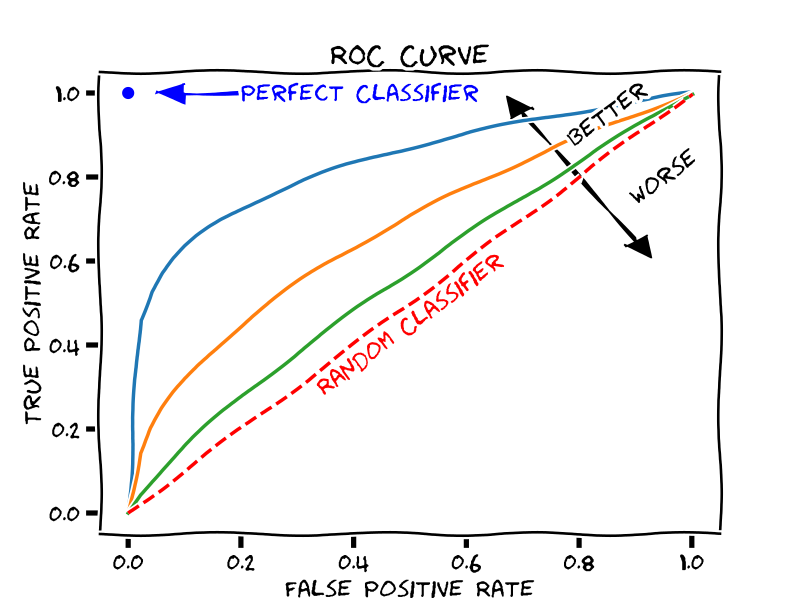
\includegraphics[scale=0.3]{roc_curve}
	\caption{ROC (receiver operating characteristic) curve examples; from \href{https://en.wikipedia.org/wiki/Receiver_operating_characteristic}{Wikipedia}.}
\end{figure} 

\begin{figure}[H]
	\centering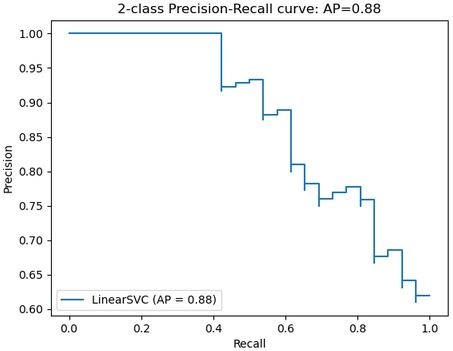
\includegraphics[scale=0.6]{precision_recall}
	\caption{Precision/recall curve example; from \href{https://scikit-learn.org/stable/auto_examples/model_selection/plot_precision_recall.html}{Scikit-Learn}.}
\end{figure} 

\begin{lstlisting}
from sklearn.linear_model import LogisticRegression

# binary classification

y_ = y=="Iris-setosa"
lr = LogisticRegression().fit(X, y_)
y_hat = lr.predict(X)
y_score = lr.predict_proba(X)[:,1]

from sklearn.metrics import confusion_matrix

confusion_matrix(y_, y_hat)
# C_ij:= number of observations of class i predicted to be in j

from sklearn.metrics import roc_curve, roc_auc_score, SCORERS

fpr, tpr, _ = roc_curve(y_, y_score)
plt.plot(fpr, tpr, 'bo-')
plt.show()

# multi-class classification

from sklearn.model_selection import cross_val_score

lr = LogisticRegression().fit(X, y)
y_scores = lr.predict_proba(X)
roc_auc_score(y, y_scores, multi_class='ovr')
cross_val_score(lr, X, y, scoring="roc_auc_ovr")
\end{lstlisting}

\end{document}
